\chapter{Ion Trap Apparatus}
\minitoc
% Main points:
    % Give a working overview of the apparatus.
    % The desired audience here is 
        %   i) Future members of FastGates, 
        %  ii) Anyone building a similar experiment, 
        % iii) Readers of other chapters who want technical detail of the apparatus.
    % Block diagram of the system
% Pre reqs:
    % Motivation for why we want this apparatus!

    A vast effort is spent on the initial build-up of the ion trap system, but
    throughout the life of the experiment, a greater effort is spent on its daily
    maintenance.  I hope that this chapter will serve as a useful debugging-resource for future
    members of the FastGates team, and as a detailed recipe for anyone
    building a similar system. \\

    Due to the size and complexity of the system, in this chapter we introduce an overview of
    the design, motivated by the desired functions.  
    Many such  ion trap experiment overviews exist in the theses of previous PhD
    generations, and so we will limit the discussion here to the unique features
    and capabilities of our system.\\
    As a map for this section we state the landmark features of an ``ion trap''
    experiment. First, to confine the ions, static and dynamic electric fields
    are used which, due to ions possesing non-zero electric charge, can provide
    trapping potentials, section~\ref{sec:The Ion Trap}. Due to the fragility of
    the internal states of the ion (these are state -of-the-art sensors after
    all), we must take great care in isolating the ion from any noisy
    environment. This neccesitates the use of ultra-high vacuum (UHV) systems,
    section~\ref{sec:Vacuum System}, vibration isolation, and magnetic
    shielding, section~\ref{sec:Magnetic Field}. To manipulate the internal
    electronic states of the ion, local electric and magnetic fields
    are created using RF antennae and, in this work, lasers, sections~\ref{sec:Laser
    systems} and~\ref{sec:Narrow Line Width 729 Laser}.  Finally, to interface
    with the apparatus we have built, at the time scales set by our interaction
    strengths, we require a sophisticated and custom control system.



\section{The Ion Trap}
\label{sec:The Ion Trap}
% Main points:
    % Introduce the NPL trap chip and its advantages
    % Short intro into the parts of the ion trap DC/RF fields.
    % Trap package CAD
    % Solidworks models of CAD with labels
    % Fastino channels
    % Experimental parameters for stable trapping
    % Quote the values we use for trapping/experiment
% Pre reqs:
    % Motivation for trapping an ion!

    \begin{figure}
        \begin{center}
        \noindent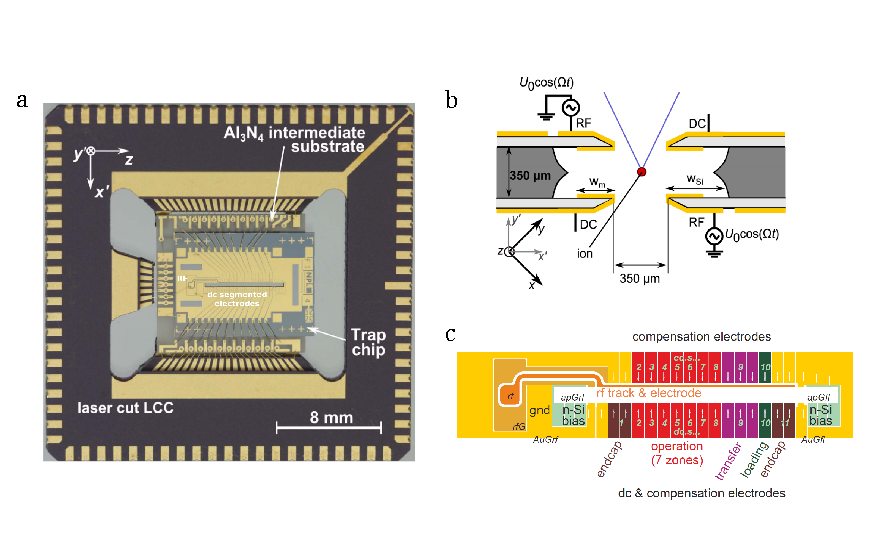
\includegraphics[width=\linewidth]{figures/pdf_figure/NPL_trap.pdf}
        \end{center}
        \caption{
            Schematics of the \emph{NPL} trap chip used in this experiment.
            \textbf{a)} A front view of the trap chip. Axial confinement is provided by a subset of the segmented DC electrodes. Radial confinement is provided by the RF rails. 
            \textbf{b)} A slice view of the trap. The red point here represents the ions, the gold are the RF and DC electrodes, and the grey is the silica substrate. It can be seen that the ion is $\sim 250 \mu$m away from the nearest electrode. The numerical aperture of the ion due to the electrodes is $\sim 0.71$.
            \textbf{c)} A schematic of the electrode geometries and labelling for the front-face of the trap chip. A similar arrangement exists for the back-face. 
            Figures from~\cite{choonee_silicon_2017}.
        \label{fig:trap}}
    \end{figure}

    From Earnshaw's theorem,
    $\nabla^2 V = 0,$ a stable stationary point in 3D cannot be realised
    using only static electric potentials, $V$, as if the potential is confining
    in two dimensions, it will be anticonfining in the third. Therefore, to
    achieve stable trapping, either an oscillating electric field (Paul
    trap~\cite{paul_electromagnetic_1990}), or a static magnetic field (Penning trap~\cite{}) is
    used.\\
    Recently, the microfabricated surface style linear Paul trap has gained
    popularity due to the maturity of chip fabrication
    technologies~\cite{allcock_surface-electrode_2011} and the potential route
    to scalability this offers~\cite{kielpinski_architecture_2002}. In the surface trap, the 3D radial and axial
    electrodes of a ``macro'' trap are effectively projected onto a 2D surface.
    The stable confining point of such a trap is typically on the order of $50-100$ $\mu$m
    above the chip surface. The ease of fabrication of surface traps has allowed
    the creation of complex multizone devices with many DC electrodes.  These
    multizone traps enable the shuttling of ions, a requirement for Quantum CCD
    type architectures~\cite{kielpinski_architecture_2002}. However, this
    surface style geometry typically comes with two costs: the depth of the
    trapping potential is often greatly reduced, and the close proximity of the
    surface to the ion can be a large contributor to motional heating
    rates~\cite{turchette_heating_2000}. \\
    Our trap is provided by the \emph{National Physical Laboratory} in the UK. This is a microfabricated 3D trap, which brings together the
    advantages of chip fabrication as well as the low heating rates and high
    trapping depths of a 3D style trap with greater ion-surface distances. Details on its design and characterisations can be found in~\cite{see_fabrication_2013,
    wilpers_monolithic_2012}. Figure~\ref{fig:trap} shows the electrode geometry of the trap and the relevant length scales.
    The ion-surface distance is now of the order $250$ $\mu$m and we have
    demonstrated heating rates of $ 33(3)$~q/s on a 4~MHz radial mode (see
    section~\ref{sec:Heating}).\\
    An axial ion separation of $\sim 5$~$\mu$m is desired. For
    $^{40}$Ca$^{+}$ ions this means an axial mode frequency of $\omega_z \approx 2\pi
    \cdot 1.6$~MHz. This ion separation was chosen as a balance between the
    desire for high mode frequencies while keeping cross talk due to
    laser-addressing negligible.\\ The mode frequencies that can be achieved are
    ultimately limited by the breakdown voltage of the trap electrodes, $V_{\rm
    MAX} = 400$~Vpp. Within this constraint, we are targeting $\sim 4$~MHz for
    our radial frequencies. The choice of this higher frequency is motivated by
    several factors: the Doppler cooling limit is reduced, and the frequency
    separation between modes can be increased, which is useful for simplifying
    interactions involving motion.\\ 
    In the following two sections we describe the experimental parameters used
    in our apparatus to achieve these mode frequencies.\\

    %Figure like Milne would be nice here - but showing zig-zag for 5 ions is hard...

    %Using the pseudopotential approximation~\cite{madsen_planar_2004} for the
    %confining field, we can find a trapping frequency in one radial direction
    %$\omega_p$
    %\begin{equation}
    %\omega_p = \frac{e\alpha V_{RF}}{\sqrt{2}\Omega_{RF}M\rho^2},
    %\label{eq:pseudopotential}
    %\end{equation}
    %where $\alpha$ is a factor of order unity given by the geometry of the trap,
    %$V_{RF}$ and $\Omega_{RF}$ are the voltage and frequency provided to the
    %RF-electrode, $M$ is the mass of the ion, and $\rho$ is the ion-RF electrode
    %separation.  Applying some DC voltage on the axial electrodes leads to axial
    %confinement with frequency $\omega_{ax}$, but must defocus the radial
    %confinements as the total curvature of the pseudopotential must remain
    %constant,
    %\begin{equation}
    %\omega_{rad} = \sqrt{\omega_p^2 - \omega_{ax}^2/2}.
    %\end{equation}
    %Due to the geometry of the DC electrodes with respect to the ion chain, the
    %\emph{NPL} trap focuses one of the radial modes and defocuses the other when
    %the DC electrodes are increased,
    %\begin{equation}
    %\omega_{rad\pm} = \sqrt{\omega_p^2 - (1\mp\beta)\omega_{ax}^2/2},
    %\end{equation}
    %where $\beta$ is some factor due to the geometry of this geometry. From
    %simulation $\beta > 1$ for $\Omega_{RF} = 2\pi\cdot 23$~MHz and $V_{RF} =
    %200$~V and so one radial mode increases with DC voltage applied and one
    %decreases.

    %\begin{table}[h!]
    %\begin{center}
    %\begin{tabular}{ c|c c c c c }
    %& $V_{RF}$/V &  $V_{DC}$/V &$\Omega_{RF}$/($2\pi\cdot$MHz)& $\omega$/($2\pi\cdot$MHz)   & q \\ 
    %&  &  & & $\omega_{ax}$\quad   $\omega_{rad}$ &  \\ 
    %\hline
    %Experiment  & 200 & -7 &  23 & 1.6 \quad 4.9 & 0.61 \\
    %Loading  & 100 & -2 &  23 & 0.8 \quad 2.0 & 0.25 \\
    %\end{tabular}
    %\caption{ Simulated trapping parameters for both ``Experiment'' and ``Loading'' settings \textsuperscript{40}Ca\textsuperscript{+} with the NPL trap. The ``Experiment'' setting is optimized for high axial mode frequencies whilst the ``Loading'' setting maintains a lower q factor for practical loading.  \label{table:freqs}}
    %\end{center}
    %\end{table}

    %A possible set of parameters to achieve $\omega_{ax} = 2\pi \cdot 1.6$~MHz
    %and $\omega_{rad+} = 2\pi \cdot 4.9$~MHz can be seen in the ``Experiment''
    %trapping in Table~\ref{table:freqs}.

    %From the Mathieu equations, the areas of stability depend upon a factor
    %$q$~\cite{berkeland_minimization_1998}, where
    %$q=2\sqrt(2)\omega/\Omega_{RF}$.  Generally, we require $q$ to be as low
    %($q<0.3$) for convenient trapping.  To satisfy this requirement a
    %``Loading'' setting (with parameters in table~\ref{table:freqs}) may be used
    %with $q = 0.25$ and then the $V_{RF}$ ramped to the ``Experiment'' trapping
    %for high radial mode frequencies.

\subsection{Trap RF Chain}
\label{sec:Trap RF Chain}
% Main points:
    % Maybe a figure describing the elements within the RF chain
        % Frequency source (Urukul)
        % Resonator
        % RF rails
    % Quote values we use.
% Pre reqs:
    % NPL trap geometry
    To utilise radial motional modes for low error quantum gates, we require the
    radio frequency (RF) field that produces the desired trapping
    pseudopotential to be both frequency and amplitude stable. Our \emph{NPL}
    trap is rated for a max peak-to-peak voltage of 400~Vpp on the RF
    electrodes. Here we describe the elements of the ``RF chain'' that supplies
    this voltage. \\
    Our frequency source is a DDS-based synthesiser, named \emph{Urukul}, part
    of the \emph{Artiq Sinara}~\cite{} hardware ecosystem. The
    \emph{Urukul} is operated at maximum output power, +10~dBm, and with a frequency $\sim 27.8$~MHz. This
    signal is then fed to an ``ultra-low noise limiting amplifier'' named
    \emph{Squareatron}~\cite{}. The purpose of \emph{Squareatron} is to
    greatly reduce the amplitude noise of the RF signal, $V_{\rm RF}$, which is
    key to low radial mode frequency drifts, as radial mode frequency $\omega_{x,y} \propto V_{\rm RF}$~\cite{}. The \emph{Squareatron} outputs +17.4~dBm,
    which is subsequently attenuated by 19.5~dB. The signal is then amplified by a
    further 33.7~dB using a \emph{Mini-Circuits ZHL-1-2W-S+}, high power
    amplifier. The signal is now +32 dBm RF power, enough to drive the trap
    electrodes. To impedance match the 50~$\Omega$ line from the amplifier to
    the small capacitance ($\sim 5$~pF) of the trap electrodes, an LC
    impedance matching circuit is used. This LC circuit has a tuned resonant frequency of 27.84~MHz, and a
    measured Q factor of 43.8 found using a vector network analyser and fitting S11 impedance measurements.
    This resonant matching circuit has three main effects: it ensures good power transfer
    between RF input and trap electrodes via impedance matching, it steps up the
    voltage to the required 400~Vpp, and it filters out RF noise and unwated harmonics due to
    the narrow bandpass nature of the LC circuit. \\
    If components are chosen well, and adequately protected from
    environmental noise, this chain can produce the desired frequency and
    amplitude stable RF. Characterisations of the motional mode
    stability are discussed in section~\ref{sec:Motional Mode Stability}. We are
    still yet to fully quantify and debug the motional stability against thermal
    and mechanical noise, however it should be noted that other groups do opt
    for active stabilisation of RF amplitude through closed feedback loops~\cite{}.\\
    % Milne sydney trap RF chain 

\subsection{Trap DC Voltages}
% Main points:
    % Describe Fastino DAC and the available electrodes on the NPL trap
    % Quote values we use.
% Pre reqs:
    % NPL trap geometry
    Voltage is supplied to the 40 DC electrodes using \emph{Fastino}, a
    multi-channel DAC part of the \emph{Artiq Sinara} hardware
    ecosystem~\cite{}.\\
    The ion is confined in the ``operation'' zone, seen in
    figure~\ref{fig:trap} c. The axial trapping is provided by electrodes
    DC-b5 and DC-f5, where b and f correspond to the back and front plane of the trap. 
    The DAC provides $\sim 10$~V to these electrodes to produce an axial frequency of 1.6~MHz.
    % XXX include section on compensation fields?
    
\section{Magnetic Field}
\label{sec:Magnetic Field}
% Main points:
    % Permanent magnets
    % MUMetal box
    Stable Zeeman shifts of the ion energy levels are required for long spin
    coherence times (see section~\ref{sec:Coherence}), and for low error single-
    and two-qubit gates. A permanent magnet array of Samarium Cobalt,
    Sm$_2$Co$_17$, is used in a Helmholtz configuration to create a stable magnetic
    field of 5.4~G. Samarium Cobalt was chosen for its low temperature
    coefficient of remenance, -0.03\%/K.\\
    The ion is shielded from unwanted external magnetic fields by two layers of
    3~mm thick MuMetal shielding from \emph{MagneticShields}. The factory quoted
    shielding factor is 546 for DC fields. Spin coherence time comparisons for
    the ion with and without magnetic shielding are shown in
    section~\ref{sec:Coherence}.\\

\section{Vacuum System and Beam Geometry}
\label{sec:Vacuum System}
% Main points:
    % Technical drawing of beam geometries and magnetic field to ion chain.
    % Drawing of ion trap package with high NA lenses
        % High NA sandwich
    % Standing waves at the ion
% Pre reqs:
    % NPL trap
    % Why we have Dual high NA lenses
    % Magnetic field giving Zeeman shift


\begin{figure}
  \begin{center}
   \noindent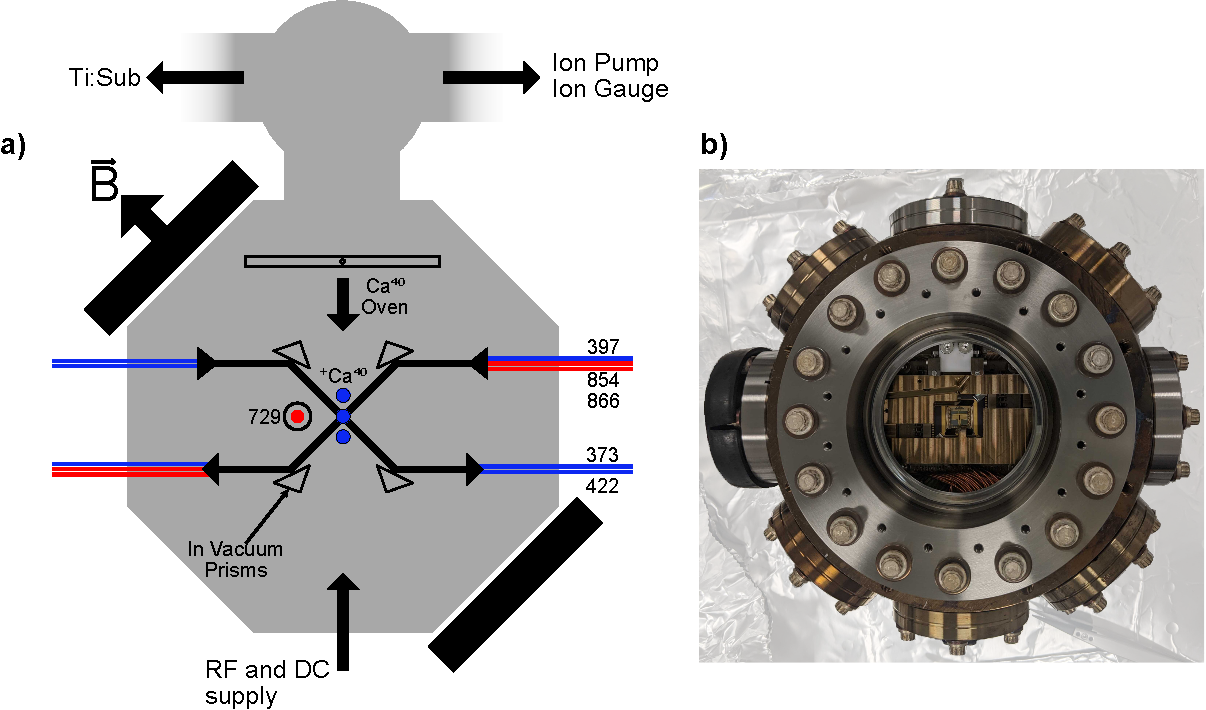
\includegraphics[width=0.9\linewidth]{figures/pdf_figure/vacuum_can-crop.pdf}
  \end{center}
  \caption{
    \textbf{a)} \mccorrect{XXX place holder figure. I would like to replace with a solidworks render.} A schematic of the vacuum chamber.
    Wavelengths apart from 729-nm enter through the side CF40 viewports and are
    directed onto the ions by in vacuum prisms. The 729-nm light enters through
    the larger CF100 viewports.  \textbf{b)} A photograph of the assembled
    system prior to baking.
  }
  \label{fig:can}
\end{figure}


\begin{figure}
  \begin{center}
   \noindent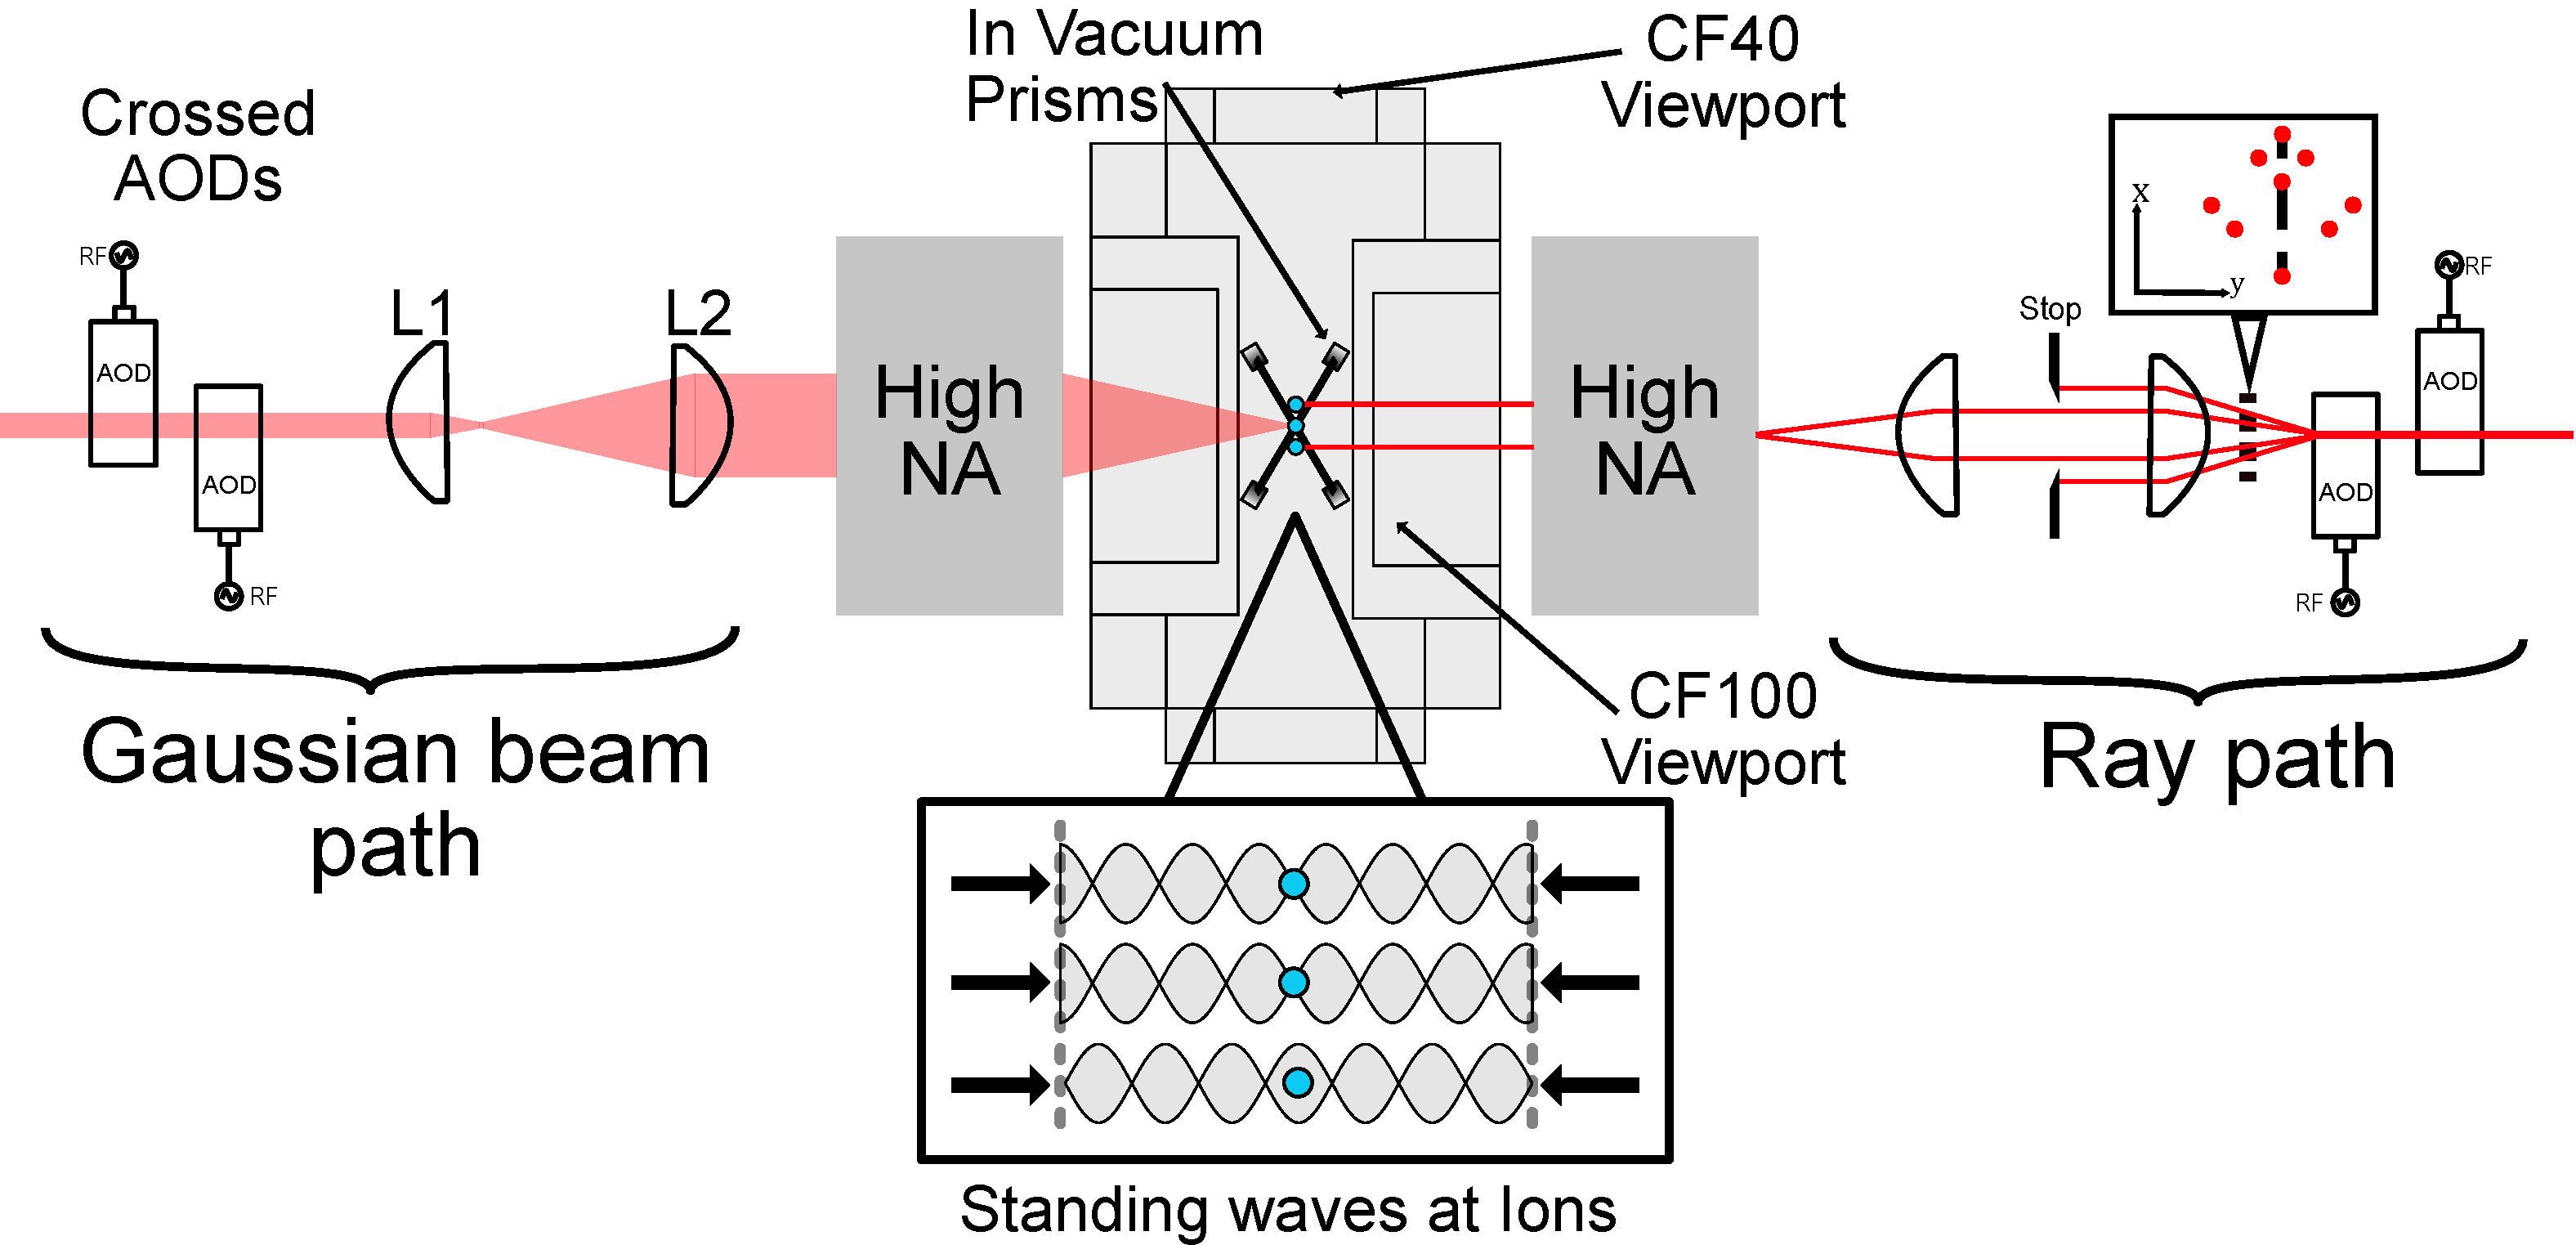
\includegraphics[width=\linewidth]{figures/pdf_figure/vac_can_AOD_small.pdf}
  \end{center}
  \caption{\mccorrect{XXX Place holder figure.} The standing wave single addressing system. Dual high NA
    objectives focus the light to a tight waist at the ions
    location. AODs are used to steer the light to only selected
    ions. The left hand side of the figure shows the Gaussian profile
    of the light, whilst the right hand side shows a ray
    representation of how two singly addressing spots are formed at
    the ions. L1 is a telecentric scanning lens and in combination
    with L2 form a beam expander.}
  \label{fig:AOD}
\end{figure}

    Ultra High Vacuum (UHV) is required to extend the ion storage lifetime.
    However, UHV equipment is often bulky, and puts constraints on the access
    and visibility of the ion chain. Here we describe the designed vacuum
    system, and beam access.  The vacuum system and beam geometries were
    designed by Sebastian Saner and Mariella Minder, and constructed by
    Sebastian Saner, Fabian Pokorny, and myself.\\
    A residual pressure of $<10^{-11}$ mbar is desired. For this strict
    requirement, care must be taken in selecting in-vacuum materials, and 
    thorough cleaning and baking procedures must be followed. A summary of tactics that were
    useful in the construction of the vacuum system can be found
    in~\cite{birnbaum_ultra-high_2005, wolf_cryogenic_2019}.\\
    A schematic and photograph of the vacuum system can be seen in
    Figure~\ref{fig:can}. The system consists of a 6" spherical-octagonal
    experimental chamber\footnote{Kimball MCF600-SphOct-F2C8} connected to a
    spherical chamber with ion pump\footnote{Agilent VacIon Plus 20 Pump}, ion
    gauge\footnote{Agilent UHV-24P Ion gauge} and Titanium sublimator pump
    (TSP)\footnote{Scanwel custom housing} attached. The ion pump and TSP
    maintain the UHV to the desired $<10^{-11}$~mbar. We find that on the ion
    pump alone UHV cannot be maintained indefinitely, however, firing the TSP
    every 4 weeks with 41~A for 60 seconds provides a sufficient pumping rate.
    At the time of system baking, a He leak test was performed, however 
    no external leaks were found. We suspect the gradual pressure increase is either due
    to our use of in-vacuum optics, optics epoxy adhesive\footnote{EPO-TEK
    353ND}, or our use of soldered PCB components.\\
    For optical access, there are two recessed CF100 viewports\footnote{UK Atomic
    Energy Authority P/N VPR100015} on the two large faces of the experiment
    can, see figure~\ref{fig:AOD}. Recessed viewports were required due to the size of the chosen main
    objectives\footnote{Photon Gear custom Atom Imager}. These custom objectives
    have an effective focal length of 33~mm, a working distance of 24.4~mm, and
    a numerical aperture, NA, of 0.6. They are coated for 397-nm and 729-nm.
    The consideration for dual high NA objectives is relatively unique in ion trap experiments, and was mainly motivated by previous work on fast entangling gates via standing waves~\cite{saner_breaking_2023}. \\
    There is further optical access via
    two CF40 side viewports\footnote{LewVac ZFSVP-DUV-40CF-OUM} coated
    for 397-nm, 422-nm, 729-nm, 854-nm and 866-nm, seen in figure~\ref{fig:can}.  Due to the spatial
    constraints from the trap assembly and high NA objectives, 
    multiple of our beams must enter the vacuum can through these side ports. For the ion chain to be visible from these side ports, in-vacuum dielectric
    mirrors are used. These fused-silica mirrors are UHV rated and coated for 372-nm, 397-nm,
    422-nm, 729-nm, 854-nm and 866-nm, with reflectivities of >99\% for both s-
    and p-polarised light. Figure~\ref{fig:can} shows a schematic of the beam
    geometries via the side ports. A limitation of this beam geometry is that due to the permanent B-field direction, it is not possible to provide pure $\pi$ or $\sigma_{\pm}$ light to the ion. However for applications where strict polarisation control is needed, the beams can be incident through the CF100 viewport.\\
    An electrical feedthrough on a CF40 flange\footnote{Allectra custom} is used to supply our trap chip and atomic source oven with DC and RF voltages. As
    the DC cables run within close proximity to the RF supply, electrical pick
    up is a potential issue for our DC lines. RF leaked onto our DC electrodes
    will create unwanted pseudopotential which can lead to unexpected mode
    geometries, or required compensation field. This leakage is mitigated through
    an in-vacuum RC low pass filter board within close proximity of the trap
    chip with a cutoff frequency of 17~kHz. The trap chip is mounted onto this
    filter board via a custom Polyether ether ketone (PEEK) interposer with
    electric feedthroughs via embedded \emph{Fuzz buttons}\footnote{Custom
    Interconnects}. \\
    % XXX seen in figure~\ref{fig:can} c.

\section{Imaging System}
\label{sec:Imaging System}
% Main points:
    % Describe the imaging system
    % Describe the camera and its properties
    % Describe the imaging optics and their properties
% Pre reqs:
    % High NA

    The imaging system is used to collect fluorescence light from the ion chain
    for readout, and to image the ion chain for characterisation.
    We aim for a separation of 5~\unit{\um} between ions, and require adequate distinguishability of ions in the imaged plane.
    The system
    consists of a high quantum-efficiency camera\footnote{Hamamatsu Orca-Fusion BT}, a f=200~\unit{\mm} relay lens, and the f=33~\unit{\mm} NA=0.6 objective. This gives a magnification of 6x, and considering the pixel size of 6.5~\unit{\um}, leads to a separation of 5 pixels between ions. The objective is on a 5-axis alignment stage with the z-axis focus controlled by a piezo micrometer for fine adjustment of the ion focus.

\section{Ca$^+$ Laser Systems}	
\label{sec:Laser systems}
% Main points:
    % State which lasers we need access to
    % Calcium level structure 
    % What frequency control do we need on each? PDH lock, AOM etc.
    % Table of all AOMs and offset frequencies
    % Table of laser powers in mW and with aimed saturation intensities for doppler idle, cooling, readout, and laser linewidths.
% Pre reqs:
    % Calcium level structure
    % 5 G field

    Singly-charged group 2 elements are popular in ion trap
    experiments due to their single outer electron resulting in Hydrogen-like
    energy levels. In this thesis we use \ca.\\
    \ca has
    no nuclear spin giving the
    (relatively) simple level structure shown in figure~\ref{fig:ion}. The external
    magnetic field of $5.4$~G is applied to split the levels via the Zeeman
    effect. The relevant laser transitions used in our apparatus are indicated.\\
    A zero nuclear spin isotope of calcium was chosen due to this simple level
    structure without hyperfine splitting. The greater number of levels due to
    hyperfine splitting lead to more decay paths and therefore greater
    complications in both cooling and gate schemes. However, due to the lack of hyperfine structure, there are no available magnetic field insensitive transitions, which are
    often used in ion trap experiments to further decouple the ion from a noisy
    environment~\cite{}. \\
    We define our qubit by the quadrupole transition at 729-nm, which we describe in section~\ref{sec:Transitions}.\\
    Access to other excited levels, outside of our defined two level system, are crucial for ion trap quantum logic to enable qubit readout via state selective fluorescence (397-nm, and 866-nm transitions), and state preparation via optical pumping (397-nm, 866-nm, and 854-nm transitions). Details on these schemes are given in chapter~\ref{ch:Characterisation}. Access to two additional transitions in neutral calcium for isotope selective ionisation, 422-nm and 372-nm, is also required~\cite{}.\\
    These transitions (apart from the 729-nm) are all driven by diode lasers\footnote{All Toptica diodes. Red lasers: MDL DL pro; Blue lasers: MDL DL pro HP; 372-nm: iBEAM-SMART-375-S}, which are frequency stabilised to a reference cavity\footnote{Stable Laser Systems SLS-6010 4-Bore Cylindrical Cavity} via Pound-Drever-Hall (PDH) locking. \mccorrect{XXX should quote finesse and FSR values here.} PDH locking is used to ensure that laser frequencies are stable to <1~MHz level, well below the natural line widths of all the dipole transitions listed above. The laser frequencies are continuosly monitored with a wavemeter\footnote{HighFinesse WS7}.\\
    Frequency and amplitude control for all lasers is achieved via acousto-optic modulators (AOMs) which are driven by Artiq integrated DDS chips, \emph{Urukuls}. The AOMs are used in a double pass configuration to allow shifts of the laser frequency by $\pm \sim 100$~MHz, with no signicant angular shifts or loss of fibre coupling. 
    
    
\subsection{Narrow Line Width 729 Laser}
\label{sec:Narrow Line Width 729 Laser} 
% Main points:
    % What equipment does the 729 consist of.
    % Solstis cavity
    % Beam path and control loops (PDH, FNC)
    % Frequency shifting, pulse carving via urukul
    % Amplitude stabilisation with SUServo
% Pre reqs:
    % Calcium level structure

    Lasers are a key tool for creating the highly localised, strong electric
    field amplitudes and gradients needed to drive both carrier and sideband
    transitions of the trapped ion.\\ As shown in Figure~\ref{fig:ion}, 
    two sublevels within the 4S\textsubscript{1/2} to 3D\textsubscript{5/2}
    manifolds define the qubit. This is an electric quadrupole transition as
    $\Delta l = 2$.  For the Calcium ion this transition is at 729-nm, and so 
    a near resonance 729-nm laser is used to implement single- and multi-qubit gates
    (sections~\ref{sec:Randomised Benchmarking} and~\ref{sec:Two-Qubit
    Entangling Gates}). This transition is also used after Doppler cooling for
    resolved sideband cooling to prepare the motional mode close to its ground
    state (as discussed in section~\ref{sec:Cooling}).
    This transition is narrrow linewidth due the the long lived
    3D\textsubscript{5/2} level, and so, for power efficiency, a
    narrow linewidth laser must be used. For the ``fast entangling gates'' use-case, high intensity electric-fields are required at the ion to drive sideband
    transitions, this will be discussed further in the single-addressing and
    two-qubit gate sections, but here it is sufficient to say we require >100 mW
    of light at the ion plane.  Here we describe the 729-nm system 
    consisting of a Ti:Sapph laser system pumped with by an Nd:YAG 532-nm laser.\\
    An \emph{M2 Solstis} Ti:Sapph~\cite{} is pumped via 18 W of 532-nm light
    from a \emph{Coherent Verdi-V} system~\cite{} to produce around 5W of
    729-nm light.  The Ti:Sapph is engineered to operate with a stable $<50$~kHz
    linewidth~\cite{}. Ti:Sapph crystals have broadband gain profiles~\cite{}, which
    are often exploited in research environments to create frequency tunable
    laser systems. We however want a narrow linewidth, single frequency laser.
    The \emph{Solstis} has multiple intracavity frequency selective
    elements which consist of (in order of coarse frequency selectivity), a
    birefringent filter, a tunable Fabry-P\'erot etalon, and the surrounding
    bow-tie cavity. For stable single mode operation, the \emph{Solstis} employs
    an active ``dither'' servo to lock the peak of etalon transmission to one of
    the cavity longitudinal mode. This dither consists of periodically varying
    the etalon spacing with a frequency of around 20~kHz. We must be aware of
    this dither frequency as the phase modulation leads to the creation of
    sidebands on our light which can interact with the ion causing unexpected
    errors in gates. This dither frequency (and harmonics of it), can be observed 
    via composite pulse experiments on the ion, however it is currently not
    expected to be a limiting source of error in any of the interactions
    we study.\\
    \begin{figure}
    \begin{center}
    \noindent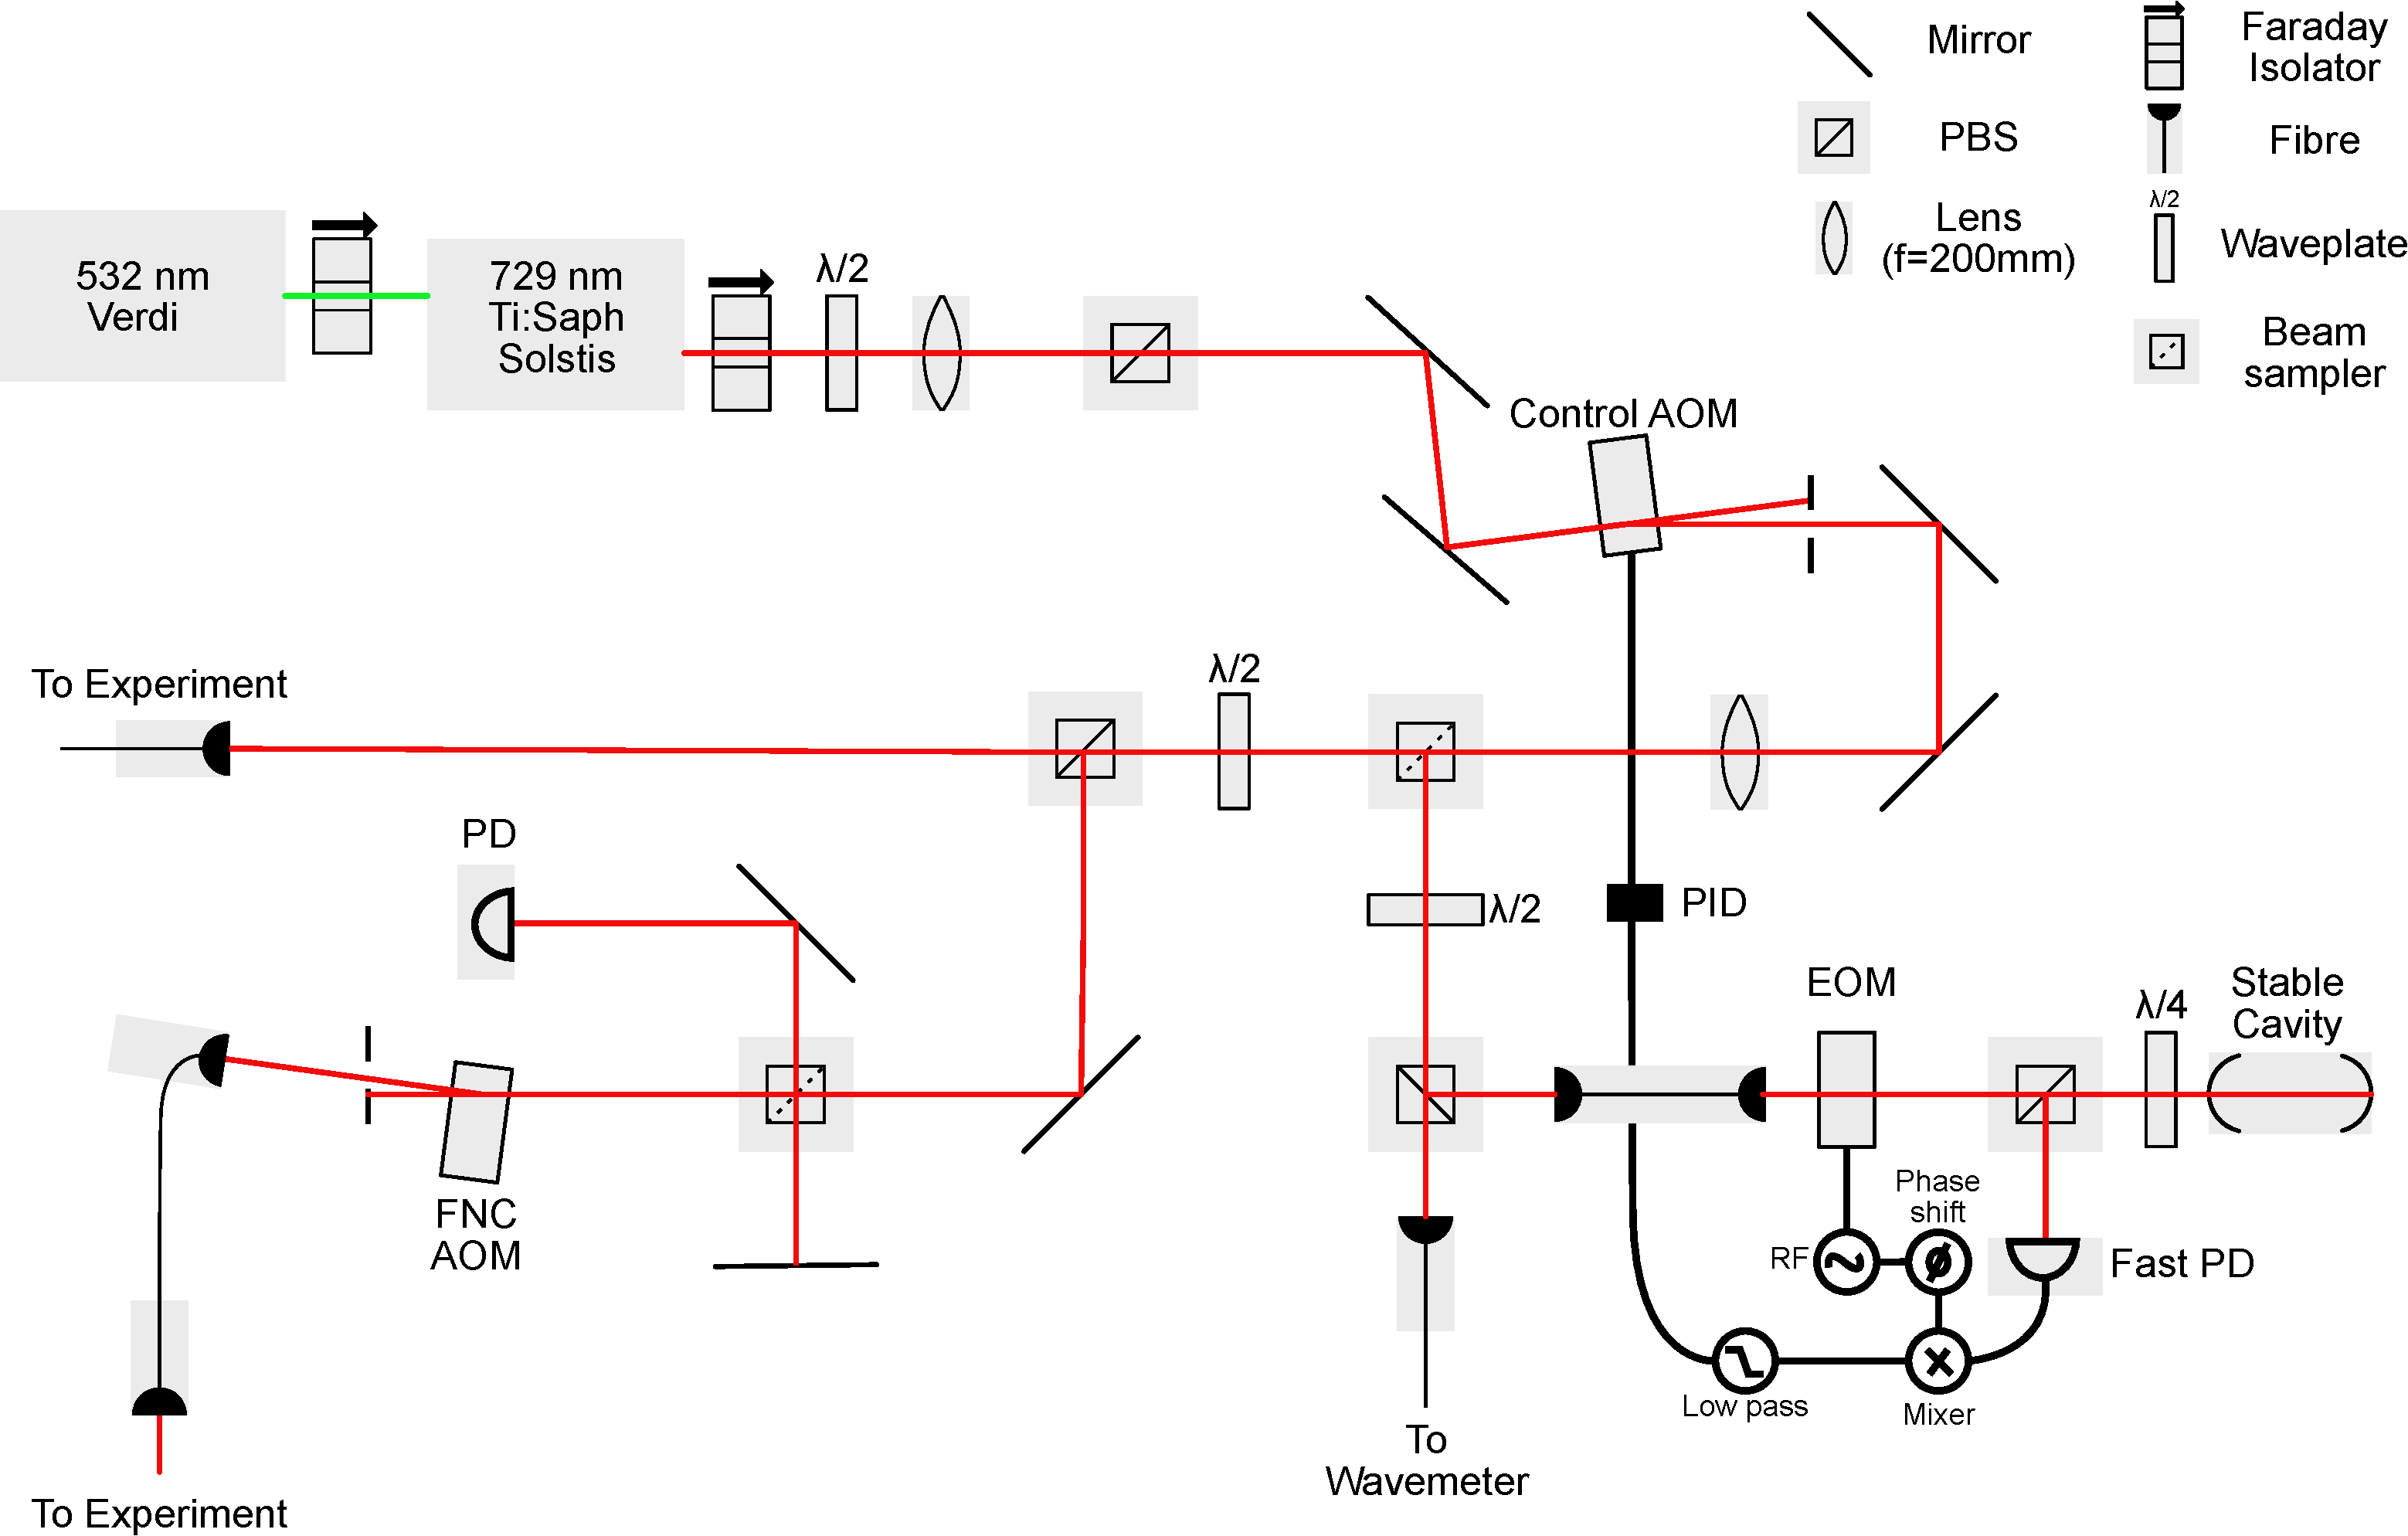
\includegraphics[width=0.9\linewidth]{figures/pdf_figure/729_path_small.pdf}
    \end{center}
    \caption{The 729-nm system. A Ti:Sapph laser tuned to 729-nm is
        pumped by a 532-nm source. Light is picked off at the first beam
        sampler to stabilise by PDH locking to a cavity.}
    \label{fig:729}
    \end{figure}
    \begin{figure}
        \begin{center}
        \noindent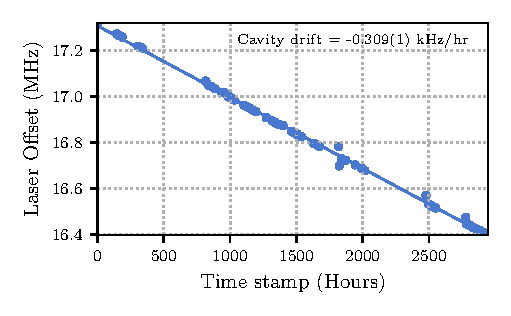
\includegraphics[width=0.75\linewidth]{
            figures/pdf_figure/cavity_drift.pdf
            }
        \end{center}
        \caption{
            Cavity drift over 125 days measured by reference to the ion transition. The laser offset here is with respect to running all 729-nm AOMs at their central frequencies. Outliers are due to bad fits of the ion transition frequency, not due to changes in the cavity resonance.
            }
        \label{fig:Cavity Drift}
    \end{figure}
    As mentioned, the \emph{Solstis} alone can operate with linewidths of
    $<50$~kHz, however this linewidth is pushed down further by referencing the Ti:Sapph output
    to an ulta high finesse cavity by \emph{Stable Laser Systems} and applying
    a Pound-Drever-Hall (PDH) lock~\cite{}. \mccorrect{XXX should quote finesse and FSR values here.} A schematic of the 729-nm system is
    shown in Figure~\ref{fig:729}.  PDH locking requires applying two sidebands
    via an electro-optical modulator (EOM) to the light and directing it onto
    the stable cavity. The light reflected from the cavity is then directed onto
    a fast photodetector\footnote{Thorlabs PDA10A2}. The reflection from the
    cavity consists of the interference between the carrier and the sidebands
    which have been respectively altered by the cavity transfer function. The
    photodetector signal is mixed down with the same oscillator signal as
    provided to the EOM but delayed by some chosen phase, and finally low pass
    filtered to produce a signal for use as the error signal in the servo loop.
    This error gives a measure for how far the carrier frequency is from the
    stable cavity resonant frequency and is used for feedback onto the control
    AOM situated after the Solstis.
    With this system, a linewidth of $<<1$~kHz for the 729-nm light is expected. 
    The electronics for this control loop are
    provided also by \emph{Stable Laser Systems} in the form of their \emph{FPGA Servo}
    lock box. For an effective PDH lock, both short and long term
    stability of the reference cavity is required. To ensure the cavity is insensitive to
    the environment, it is made of an ultra low expansion material. 
    The cavity is temperature stabilised at the zero crossing temperature of
    $30.6^\circ$C, and is further isolated by being housed in a vacuum system
    at $<1e-7$~mbar. Long term cavity drifts of 309(1) Hz/hr are measured over
    125 days, seen in figure~\ref{fig:Cavity Drift}. This measurement uses the ion as a
    frequency reference to probe the cavity frequency and is discussed in
    section~\ref{sec:Laser Offset}.\\
    Figure~\ref{fig:729} displays the other beam paths for our 729-nm system.
    Some light is picked off and sent to a wavemeter to continuosly monitor the
    frequency. However, the majority is coupled to two output fibres for our
    experiment and another within the group. The 729-nm light is transported from
    a dedicated laser lab to a the trap apparatus lab by a 10~m
    single mode polarization maintaining fibre.  The fibre is
    beneficial in cleaning up the mode from the Ti:Sapph, however it can
    introduce phase noise due to mechanical and thermal effects along the 10~m
    length. To remove this introduced noise, passive stabilisation in
    the form of thick foam tubing along the fibre length, as well as active
    stabilisation by a fibre-noise-cancellation (FNC) technique~\cite{}, is used. This
    topic has been discussed extensively in multiple PhD and Masters
    theses~\cite{}, and so here we only quote the relevant control aspects of
    our arrangement. We use the \emph{Sinara Stabilizer}~\cite{} board, a
    dual channel PID microcontroller, with the \emph{Pounder}~\cite{}
    mezzanine board, a dual channel PDH lock generator. The FNC PID software was
    developed by A. Agrawal ~\cite{}. A comparison of spin coherence times
    is shown in section~\ref{sec:Coherence} with and without fibre noise
    cancellation enabled. \\


\subsection{Single Addressing System}
\label{sec:Single Addressing System}
% This section is not used in any characterisation - could be left for outlook!
% Main points:
    % The advantages of single addressing using AODs
        % Ion selectivity
        % High intensity electric field
    % single addressing system creating standing waves
    % render of single addressing system
% Pre reqs:
    % 729 system
    % High NA
    % Trap package
    % Motivation for future experiments
    A unique feature of our system is the ability to produce single ion addressing standing waves.
    The design of this system is shown in
    figure~\ref{fig:AOD}.  A single ion addressing system must be able to
    illuminate selected ions in the crystal whilst the others remain
    unperturbed. The advantage of single addressing, other than ion selectivity,
    is the increased intensity of light due to the tight waist at the ion
    location. \\
    Our ions are separated by a distance $d\approx 5~\mu$m.  The diffraction limited radius for a
    collimated 729-nm beam with an objective lens of NA = 0.6 is $\omega_0 = 386$~nm.  Abberations present in real optical
    components will cause the addressed spot to be increasingly non-Gaussian and
    lead to unfavourable cross talk at the neighbouring ions. Therefore care was
    taken in the optical design. See I. {\O}vergaard Master thesis~\cite{} for relevant design considerations and rationale.\\
    To produce more than one addressed spot and to steer the spots along the ion
    crystal, Acousto-Optical-Deflectors\footnote{ISOMET OAD1343-XY-T70S}
    (AODs)~\cite{nagourney_quantum_2014, li_low-crosstalk_2023,
    pogorelov_compact_2021} are used. The beam deflection angle is proportional to the
    drive frequency supplied to the AOD. \mccorrect{XXX could extend this section substantially.} \\